\clearpage
\twocolumn[{%
\rqparent
\subsection{Noise and SNR}
\label{app:rq03_noise_and_snr}

\noindent\begin{minipage}[t]{0.485\textwidth}
\vspace{0pt}
\paragraph{Research Question.} \emph{How much does a measurement move when nothing but the seed or the checkpoint changes, how does that noise compare with the effect of a design decision, and what is each benchmark's signal-to-noise ratio under the 22 candidate definitions?}

\paragraph{Setup.} We measure the effect of a design decision on a task's final score against two kinds of noise, per (size, K, task) cell. The decisions are depth (deep vs shallow), data scheme A vs B, data scheme A vs C, sampling temperature T = 1 vs T = 3, activation (xIELU vs SwiGLU) and optimizer (AdEMAMix vs Muon), each against the baseline, between the seed-1904 runs of every cell, 90M--1.7B. The seed noise is the sample standard deviation of the final score across the three seeds of the replicated baseline cells (deep, scheme A: 175M and 600M at K $\in$ \{1, 2, 50\}, 1B at K $\in$ \{1, 2, 30\}). The checkpoint noise is the standard deviation of the scores around a straight line fitted to the last 20 \% of a run (the checkpoints at 80, 85, 90, 95 and 100 \%). We divide the absolute difference between the two levels of a decision by each noise and take the median over the cells. We do this separately for the benchmarks (with their rf and bBPB twins), the per-language BPB, its macro average and the training loss, and we leave out cells at chance. For the per-language BPB we count, per design axis, the (pair, language) comparisons whose 600M difference has the opposite sign of their 1.7B difference, and whether that 600M difference exceeds one seed standard deviation (Table~\ref{tab:app_rq03_flip_attribution}).
\end{minipage}\hfill
\begin{minipage}[t]{0.485\textwidth}
\vspace{0pt}
\begin{rqfinding}
\textbf{1. Seed noise exceeds checkpoint noise.} The seed std is a median 1.75$\times$ the detrended checkpoint std over 4650 ungated cells (2.04 at 175M, 1.72 at 600M and 1.53 at 1B) and is larger in 75 \% of them. (Figure~\ref{fig:app_rq03_noise_and_snr}.)
\\
\\
\textbf{2. So the checkpoint-noise SNR is optimistic.} A design difference that clears the checkpoint noise need not clear a re-roll of the seed: on the same 4562 seed cells, depth's median effect is 2.12$\times$ the detrended checkpoint noise but 1.30$\times$ the seed noise (52 \% against 30 \% of the cells above 2$\times$).
\\
\\
\textbf{3. No design axis clears twice the seed noise in half of its cells.} Against seed noise the median effect is 1.30 for depth, 1.22 for scheme A vs B (1779 cells, 29 \% above 2$\times$), 1.66 for scheme A vs C (808, 43 \%), 1.80 for temperature T 1 vs 3 (3705, 46 \%) and 1.10 for activation (1066, 27 \%).
\end{rqfinding}
\end{minipage}

\vspace{\baselineskip}
\noindent\begin{minipage}{\textwidth}
\centering
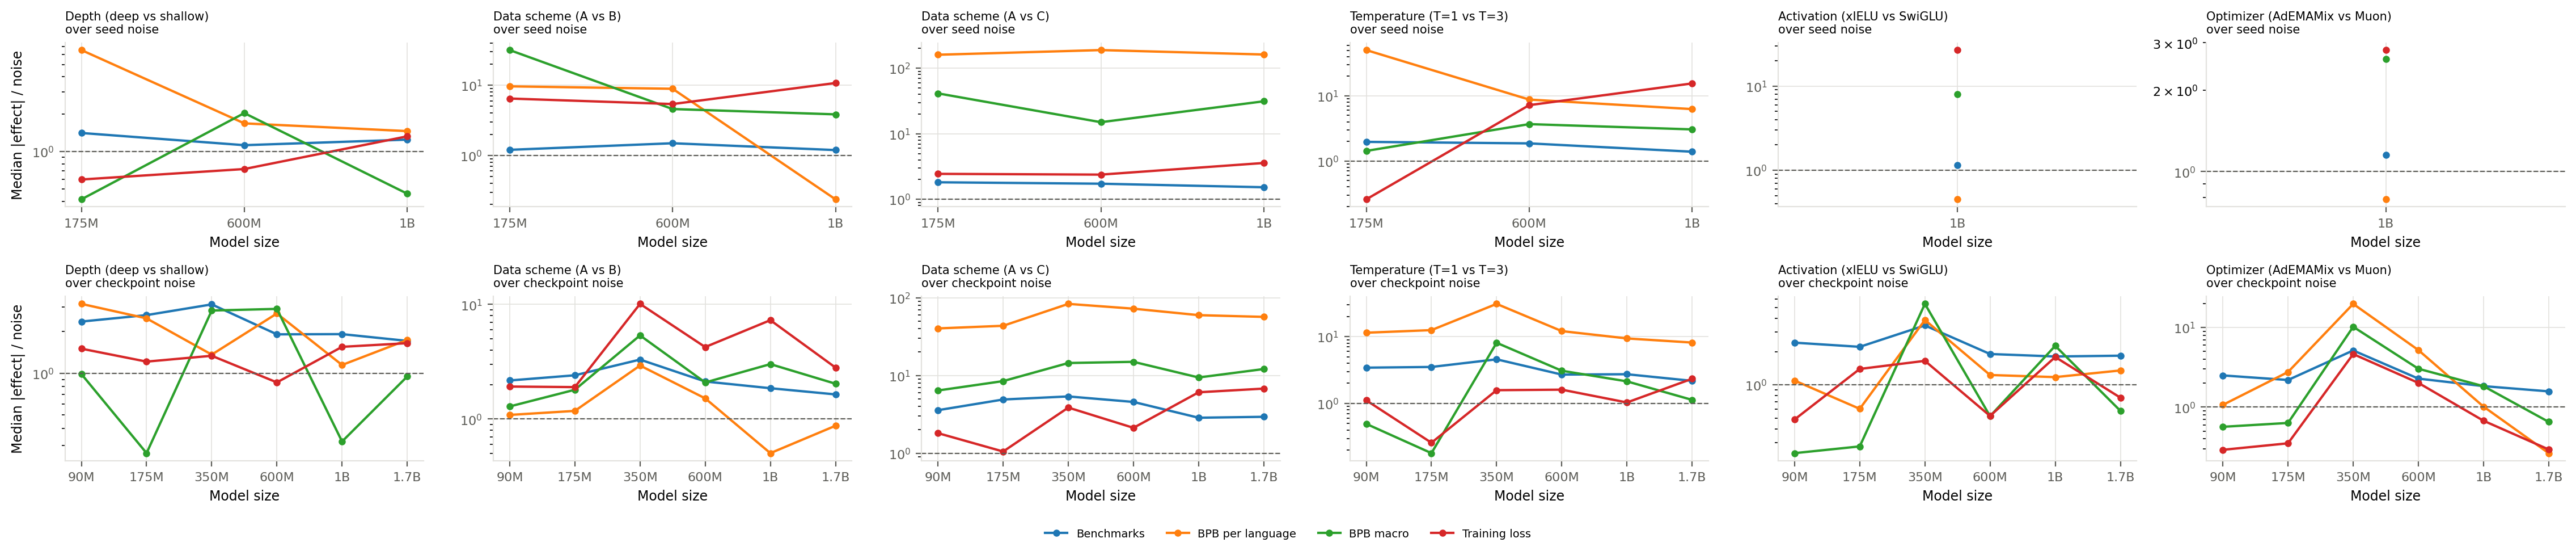
\includegraphics[width=\textwidth,height=0.36\textheight,keepaspectratio]{figures/app_rq03_noise_and_snr.png}
% source: src/signal-and-noise/analysis/rq03_noise_and_snr/pretraining/predictivity_seeds/effect_vs_noise_paper.png
\captionof{figure}{\textbf{Seed noise exceeds checkpoint noise.} Median over the (K, task) cells of a size of the absolute effect of each design decision (seed 1904, final checkpoint) over the noise, on the benchmarks (accuracy tasks with their rf and bBPB twins), the per-language bits per byte, the macro average of the bits per byte and the training loss. Top row: over the seed noise, only at the nine replicated cells (175M, 600M, 1B), so activation has only 1B (K = 30) and the optimizer a single cell (the training loss at 1B). Bottom row: over the checkpoint noise of the baseline run, 90M--1.7B. Muon has only the training loss at 1B and 1.7B. There is one column per decision. The dashed line at 1 is where the effect equals the noise (log scale). A pure seed re-roll would reach a median of 1.15 in the top row.}
\label{fig:app_rq03_noise_and_snr}
\end{minipage}
}]

\begin{table*}[p]
\centering
\small
\begin{adjustbox}{max width=\textwidth}
\begin{tabular}{lcrrrrrrrrr}
\toprule
 & Size & & & \multicolumn{2}{c}{Share (\%)} & \multicolumn{4}{c}{Cross tab (\% of comparisons)} & \\
\cmidrule(lr){5-6}\cmidrule(lr){7-10}
Design axis & matched & Pairs & Comparisons & (a) & (b) & (a), (b) & (a), not (b) & not (a), (b) & not (a), not (b) & (a), (b), 1.7B clear \\
\midrule
Depth (deep vs shallow) & no & 10 & 209 & 42 & 95 & 41 & 1 & 54 & 4 & 64 \\
Language count & yes & 45 & 378 & 74 & 15 & 3 & 71 & 12 & 14 & 1 \\
Data scheme (A vs B vs C) & yes & 12 & 80 & 39 & 2 & 1 & 38 & 1 & 60 & 0 \\
Temperature (T=1 vs T=3) & yes & 4 & 145 & 92 & 1 & 0 & 92 & 1 & 7 & 0 \\
Activation (XIELU vs SwiGLU) & yes & 3 & 53 & 21 & 83 & 19 & 2 & 64 & 15 & 6 \\
Optimizer & yes & 3 & 53 & 100 & 70 & 70 & 30 & 0 & 0 & 0 \\
\midrule
All mono-axis pairs & no & 77 & 918 & 65 & 37 & 16 & 49 & 21 & 14 & 71 \\
\midrule
Multi-axis pairs & no & 496 & 4299 & 80 & 21 & 10 & 70 & 11 & 9 & 147 \\
Multi-axis, depth moved & no & 220 & 2040 & 78 & 29 & 13 & 64 & 15 & 7 & 119 \\
Multi-axis, depth held & yes & 276 & 2259 & 82 & 14 & 7 & 75 & 7 & 11 & 28 \\
\bottomrule
\end{tabular}

\end{adjustbox}
% source: src/signal-and-noise/analysis/rq03_noise_and_snr/pretraining/predictivity/flip_attribution_da_size_by_axis_both_axes.tex
\caption{\textbf{At 600M, per-language BPB misses the 1.7B decision mostly on the depth pairs, which are not size-matched.} One row per design axis (single-axis pairs) and for every design pair (the multi-axis set, single-axis pairs included), split by whether the pair moves depth. A comparison is one design pair on one of the 50 per-language BPB tasks, between the final checkpoints of seed 1904 at 600M and at 1.7B. (a): the 600M difference exceeds one 600M seed standard deviation of the task, the median over the deep three-seed cells of the baseline data (the K = 50 cell alone for 48 of the 50 languages). (b): its sign differs from the sign of the 1.7B difference. (b) without (a) means that the 600M comparison cannot distinguish the variants, (a) with (b) that the design choice has opposite measured effects at the two sizes. The last column counts the (a), (b) comparisons whose 1.7B difference also exceeds that deviation. A difference of two runs has a seed standard deviation of 1.41 times that of one run, so (a) admits about half of the pure seed differences. At that 1.41 threshold the last column falls from 64 to 13 for depth. The optimizer axis has no per-language BPB pair at both sizes.}
\label{tab:app_rq03_flip_attribution}
\end{table*}
